O STM32F103C8, também conhecido como Blue Pill, é um microcontrolador fabricado
pela STMicroelectronics, de 32-bits. Tem como processador o ARM Cortex-M3, de
64Kbs de memória flash. O processador Cortex-M3, projetado pela ARM (Advanced
RISC Machine Ltd.) é  baseado em arquitetura Harvard, de 32-bits. A família de
microcontroladores STM32 fornece base para uma uma grande variedades de
sistemas embarcados, e com custo inferior e maior flexibilidade quando comparado
ao Arduino com ATmega, que possui microcontroladores de 8 a 16bits. Contudo,
essa flexibilidade e baixo custo têm como contrapartida o requerimento de um
maior nível de experiência em programação C do que o necessário para
desenvolver as mesmas soluções em Arduino (cuja concepção teve como objetivo
maior acessibilidade para iniciantes \cite{cortex_m3}).

O STM32F103C8 possui 7 timers, 2 ADCs, e 9 interfaces de comunicação, incluindo
I2C (\textit{Inter-Integrated Circuit}), USART (\textit{Universal Synchronous
Asynchronous Receiver Transmitter}), SPI (\textit{Serial Peripheral Interface}),
CAN e USB 2.0.


\begin{figure}[h]
	\centering
	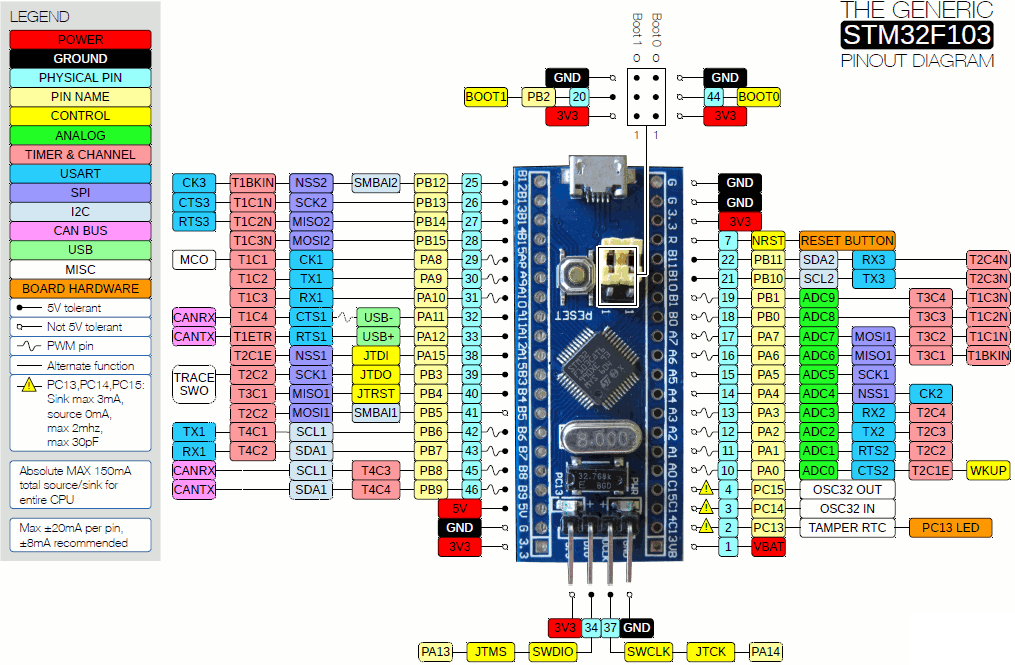
\includegraphics[width=1.0\textwidth]{figures/stm32f1_pinout}
	\caption{Diagrama de pinos do STM32F103C8}
\end{figure}

